\documentclass[11pt]{article}
\usepackage{acl2015}
\usepackage[utf8]{inputenc}
\usepackage{times}
\usepackage{url}
\usepackage{latexsym}

\usepackage{makecell}
\usepackage{pbox}
\usepackage{color}
\usepackage{graphicx}

\setlength\titlebox{6cm}

% You can expand the titlebox if you need extra space
% to show all the authors. Please do not make the titlebox
% smaller than 5cm (the original size); we will check this
% in the camera-ready version and ask you to change it back.


\title{Linghub: Aggregated Metadata about Language Resources as Linked Data}

\author{John P. McCrae, Philipp Cimiano \\
  CIT-EC, Bielefeld University \\
  Bielefeld, Germany \\
  {\scriptsize\tt\{jmccrae, cimiano\}@cit-ec.uni-bielefeld.de}}
%\\
%  {\bf Victor Rodr\'iguez Doncel, Daniel Vila-Suero}\\
%  {\bf Jorge Gracia} \\
%  Universidad Polit\'ecnica de Madrid \\
%  Madrid, Spain \\
%  {\scriptsize\tt\{vrodriguez, dvila, jgracia\}@fi.upm.es} \\\And
%  Luca Matteis, Roberto Navigli \\
%  University of Rome, La Sapienza \\
%  Rome, Italy \\
%  {\scriptsize\tt \{matteis, navigli\}@di.uniroma1.it} \\
%  {\bf Andrejs Abele, Gabriela Vulcu}\\
%  {\bf Paul Buitelaar} \\
%  Insight Centre, National University of Ireland\\
%  Galway, Ireland \\
%  {\scriptsize\tt \{andrejs.abele, gabriela.vulcu,}\\
%  {\scriptsize\tt paul.buitelaar\}@insight-centre.org} \\}
 
\date{}

\begin{document}
\maketitle
\begin{abstract}
    Abstract.
\end{abstract}

\section{Introduction}

Language resources are essential for nearly all tasks in natural language
processing (NLP) and in particular
for the adaptation of resources and methods to new domains and languages. In
order to use language resources for new purposes they must first be discovered
and this can only be done if there is a comprehensive list of all resources that
may be available. To this there have been a number of projects that have
attempted to collect such a catalogue using various methods and with differing
degrees of data quality. We present a new portal, Linghub, that aims to integrate all
these data from different sources by means of linked data and thus to create a
portal, whereby all information about language resources can be included and
queried using a common methodology. As such, this resource will enable wider
discovery of language resources for researchers in NLP, computational
linguistics and linguistics.

Currently, the approaches to metadata collection can be split into two broad
classes: firstly, \emph{curatorial} resources, which are those for which collections of
language resources are maintained by one or more institute. Such resources have
an advantage in that such metadata is normally of very high quality, however the
resulting data often fails to cover the whole spectrum of data available.
Examples of this include the META-SHARE~\cite{federmann2012meta} project and the
CLARIN project's Virtual Language Observatory~\cite[VLO]{van2012semantic}. On
the other hand, \emph{collaborative} approaches rely on data publishers
self-reporting data about their own language resources. This can be advantageous
as it allows reporting by researchers not directly collected to existing
infrastructure projects, however the resulting data is often of lower quality as
the systems may use free-text input or tagging input rather than controlled
vocabularies, as they are easier for non-expert users to understand.

Given the nature of this difference we wish to make data available from multiple
sources in a homogeneous manner and to this end we adopted a model based on the
DCAT data model~\cite{maali2014data} along with properties from Dublin
Core~\cite{weibel1998dublin}. In addition, we used the RDF
version~\cite{mccrae2015ontology} of the META-SHARE
model~\cite{gavrilidou2012meta}, to provide for metadata properties that are
specific to language data and linguistic research. As such, in this paper we
describe the creation of the largest collection of information about language
resources and briefly describe its publication on the Web by means of linked
data principles.

The rest of the paper is structured as follows...

\section{Related Work}

\section{Extraction of data}

\begin{table}
	\centering
	\begin{tabular}{p{30mm}|cc}
	Source               & Records    & Triples  \\
	\hline
	Datahub              &            &          \\
	META-SHARE           &            &          \\
	LRE-Map              &            &          \\
	CLARIN VLO           &            &          \\
	\hline
	All                  &            &          \\
	\end{tabular}
	\caption{Size of Linghub dataset by source\label{tab:size}}
\end{table}

In order to ensure that all the data from many sources can be queried in a
homogenous manner we had to convert them to RDF. This process is also proved to
be a valuable opportunity to align these vocabularies with standard vocabularies
and fix any modelling errors. Two of our resources, LRE-Map and Datahub, were already available in RDF
and thus, it should be the case that that the conversion of these resources
required only renaming the URLs so that they would resolve without any
collisions when uploaded to the Linghub portal. In fact, we also took this
opportunity to fix a number of quality issues, such as fixing property values to
either literals or URIs, reducing the number of blank nodes and changing
modelling to that recommended in relevant standards, such as
VOID~\cite{alexander2011describing}. 

The other resources used XML schemas, for which we needed to create a custom
conversion for each of them, which we did with the help of an invertible
transformation language similar to XSLT. For META-SHARE, this was a challenging
task as there were nearly a thousand unique tags defined and each one was
examined to see if it was similar to an existing Semantic Web vocabulary, and in
fact we ended up mapping to FOAF~\footnote{\url{http://xmlns.com/foaf/spec/}},
SWRC~\footnote{\url{http://ontoware.org/swrc/}} and the Media
Ontology~\footnote{\url{http://www.w3.org/TR/mediaont-10/}}. In the case of
CLARIN, there was actually a significant difference between the XML schemas used
by each contributing instance, with only a small common section giving the
resource title and download link. We thus developed distinct mappings for the
largest X institutes.

\section{Harmonization and duplicate detection}

\begin{table*}
	\centering	
	\begin{tabular}{p{50mm}p{50mm}|cc}
	Property     & Target             & Links        & Precision \\
	\hline
	Language     & LexVo              &              &           \\
	Type         & BabelNet           &              &           \\
	Usage        & META-SHARE OWL     &              &           \\
	Rights       & License ...        &              &           \\
	Backlink     & Original Resources &              & n/a       \\
	\end{tabular}
	\caption{Number of introduced links in the Linghub data\label{tab:links}}
\end{table*}	

Two key issues emerge when collecting data from a heterogenous set of sources 
such as we are doing. Firstly, the data is likely to be noisy and inconsistent 
in the properties it uses and more importantly in the values that these
properties have. For example, languages may be represented by their English 
names or alternatively by means of the codes such as the ISO 639 codes. Secondly,
it is often the case that a dataset may be recorded in multiple sources and thus,
we may create multiple records of the same dataset. Furthermore, we often see
duplication in the form of multiple records describing different sections of a 
single dataset or multiple usages of the single dataset. In order to remove 
these duplications we used state-of-the-art word sense disambiguation techniques, 
including Babelfy~\cite{} to identify common controlled vocabularies and duplicate
entries. For the case of properties we mapped to several existing resources, 
including LexVo~\cite{} for languages, and BabelNet for resource types. Duplicate 
entries were not removed from the dataset but instead were marked with the addition
of the Dublin Core property \emph{is replaced by}. In the case that these entries
were subsets of resources the target of this link would be a new combined record
for the entire resource and in the case of duplicate records collected from distinct
sources we referred to the most complete triple, that is the record with the most
triples.

\section{The Linghub portal}

\begin{figure*}
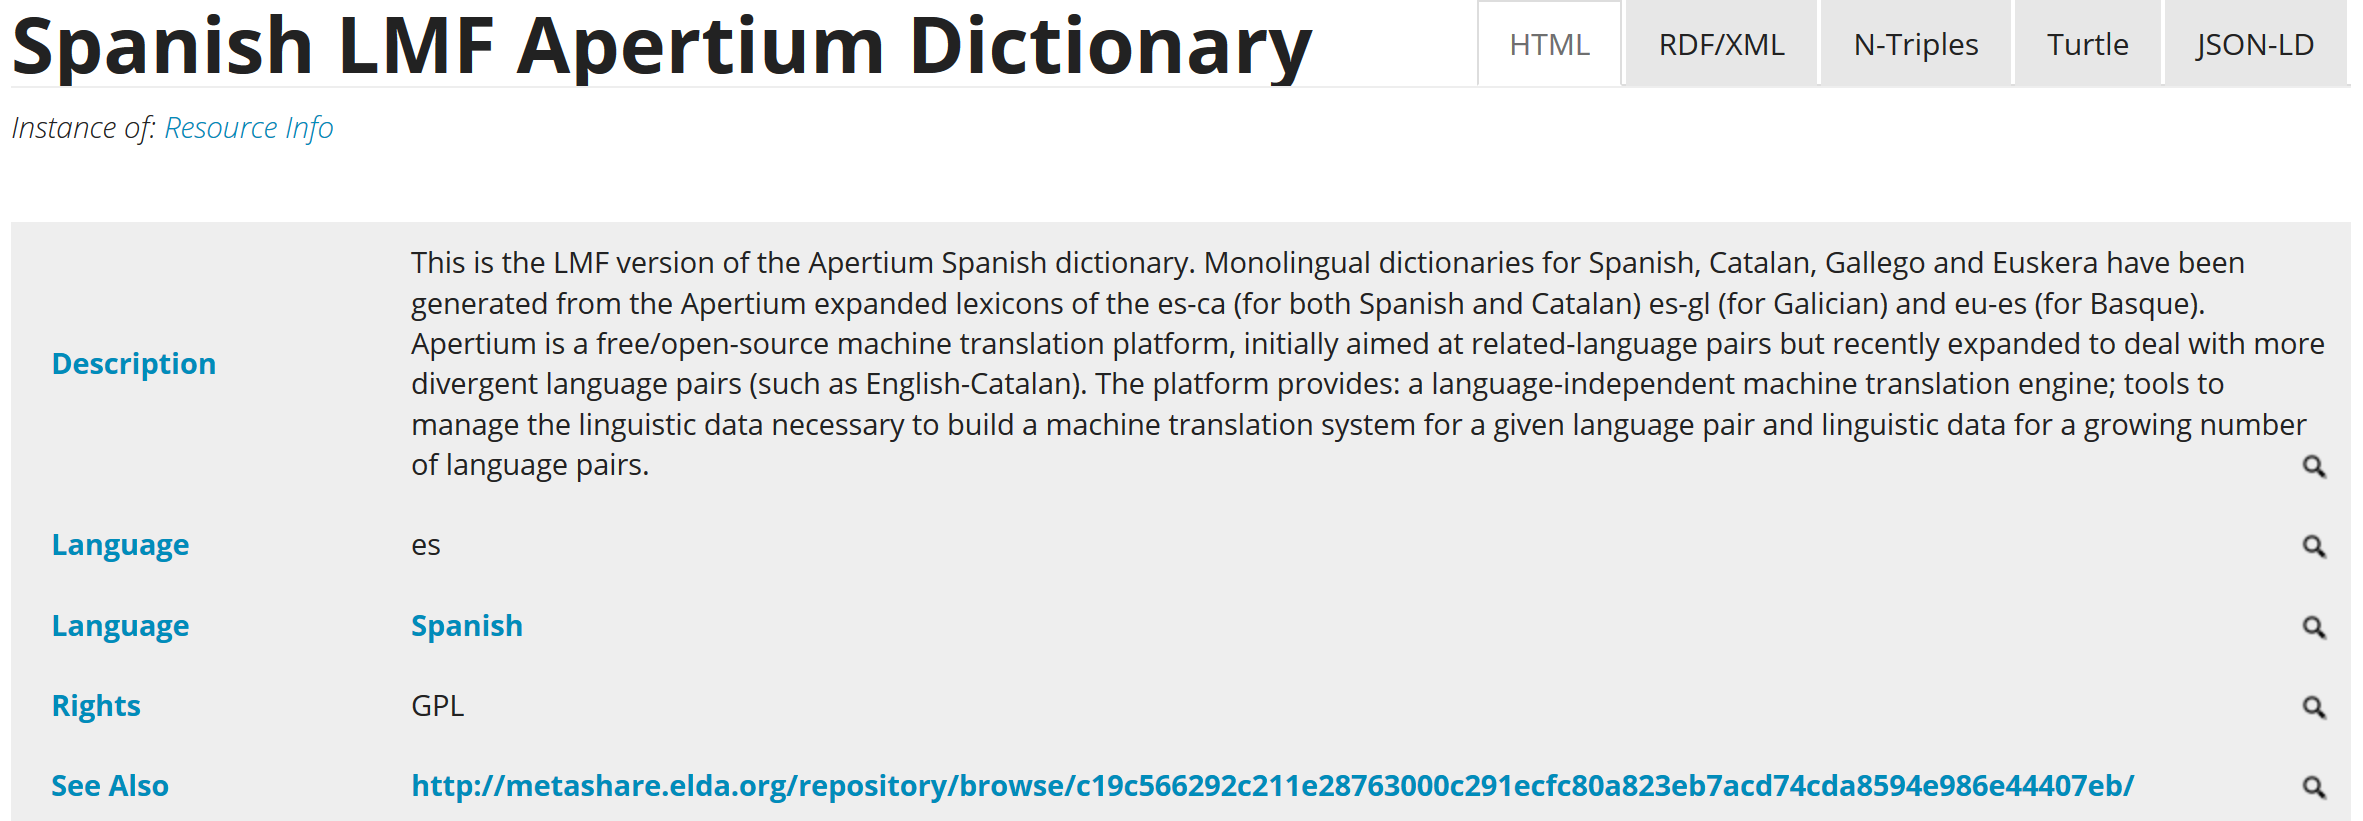
\includegraphics[width=.9\textwidth]{linghub-screenshot.png}
\caption{A screenshot of the Linghub interface\label{fig:screenshot}}
\end{figure*}

In order to enable users to quickly and easily discover datasets, we set up a 
portal for browsing the dataset. Naturally we set this up as a site that publishes
the individual records as either RDF or HTML, with the actual content delivered
to the client decided by means of content negotiation. In addition, we provide a 
number of mechanisms by which users and automated agents can discover a dataset. 
In particular, for users we allowed browsing by means of faceted browsing of 
principle aspects of datasets including language. In addition, we enabled a full
text search of the data based on the description. Machine based agents may access
the endpoint by means of SPARQL querying, although the endpoint limits the agents
to a very specific subset of the SPARQL query language. This is to ensure that 
the SPARQL querying remains stable and consistent, as full SPARQL queries could
easily destabilize the server and adding timeouts could lead to unpredictable
failures. In addition the server returns SPARQL JSON results and so can be called
easily from a web browser.


\section{Conclusion}


\section*{Acknowledgments}

%LingHub was made possible due to significant help from a large number of people,
%in particular we would like to thank the following people: Benjamin Siemoneit
%(Bielefeld University), Tiziano Flati (University of Rome, La Sapienza), Martin
%Br\"ummer (University of Leipzig), Sebastian Hellmann (University of Leipzig),
%Bettina Klimek (University of Leipzig), Penny Labropolou (IEA-ILSP), Juli
%Bakagianni (IEA-ILSP), Stelios Piperidis (IEA-ILSP), Nicoletta Calzolari
%(ILC-CNR), Riccardo del Gratta (ILC-CNR), Marta Villegas (Pompeu Fabra),
%N\'uria Bel (Pompeu Fabra) and Christian Chiarcos (Goethe-University Frankfurt).
%
%+Asun

\bibliographystyle{acl}
\bibliography{../linghub-acl15}

\end{document}
